% !TEX root = ../Dokumentation.tex
\subsection{Gesamtübersicht}

\begin{figure}[h!]%Position festigen
\centering
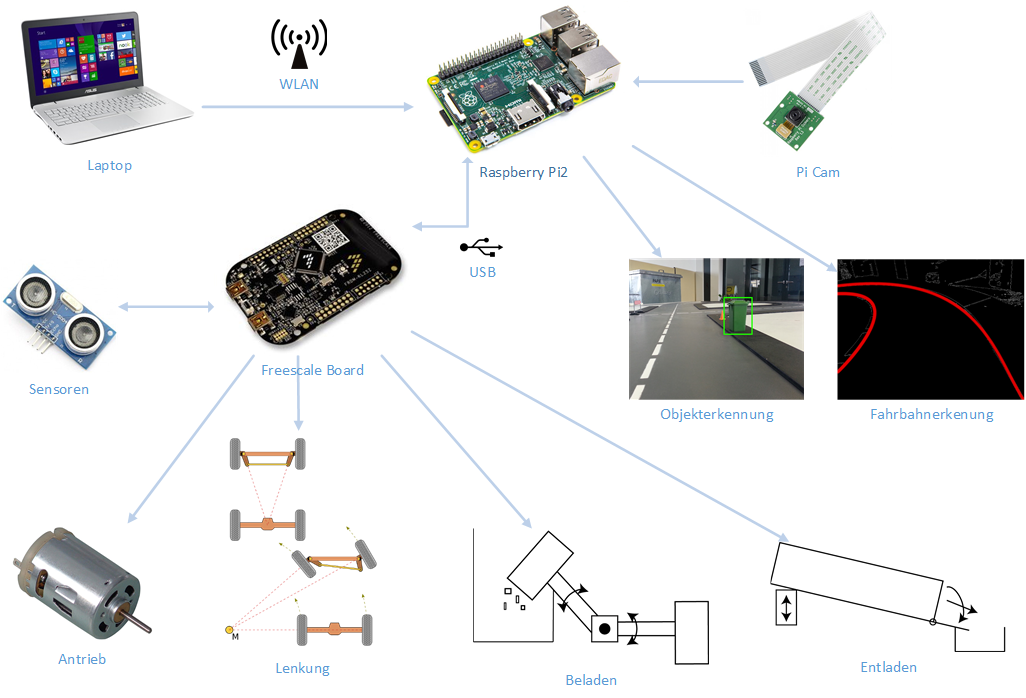
\includegraphics[width=0.9\textwidth]{03_Loesungskonzept/pictures/uebersichtszeichnung.png}
\caption{Übersichtszeichnung}
\label{fig:Java}
\end{figure}

\subsubsection{Zusammenspiel}
\textbf{Funktionsbeschrieb}\\[0.2cm]
Wie die obige Darstellung zeigt, besteht zwischen allen Komponenten ein enges Zusammenspiel.
So wird beispielsweise die gesamte Bilderkennung über den Minicomputer gesteuert.Dieser erhält seine Daten durch die Kamera und sendet die ausgewerteten Informationen an den Microntroller. Dort treffen sie mit den Messungen der Sensoren zusammen und werden ausgewertet um zu entscheiden welcher Motor angesteuert werden muss. Die Motoren wiederum, lösen die mechanischen Bewegungen aus wie z.B die Schwenkung der Kamera oder das Senken des Greifarmes.
\subsubsection{Schnittstellen}
\textbf{Funktionsbeschrieb}
\textbf{Komponentenbeschrieb}
\textbf{Begründung}
Wenn benötigt
\textbf{Berechnungen}
\textbf{Testergebnisse}